\section{量子算法设计（算法原理、步骤与伪代码）}
\subsection{算法原理}
本文算法由两部分组成：经典部分使用 LETKF 完成集合传播与局地分析；量子部分负责生成局地相似度，用于调制局地观测权重，并对集合扰动方向施加由局地耦合系数控制的弱 $J$ 修正。其设计思想是：让量子模块提供结构信息，而不是替代整个同化器。

\begin{figure}[htbp]
\centering
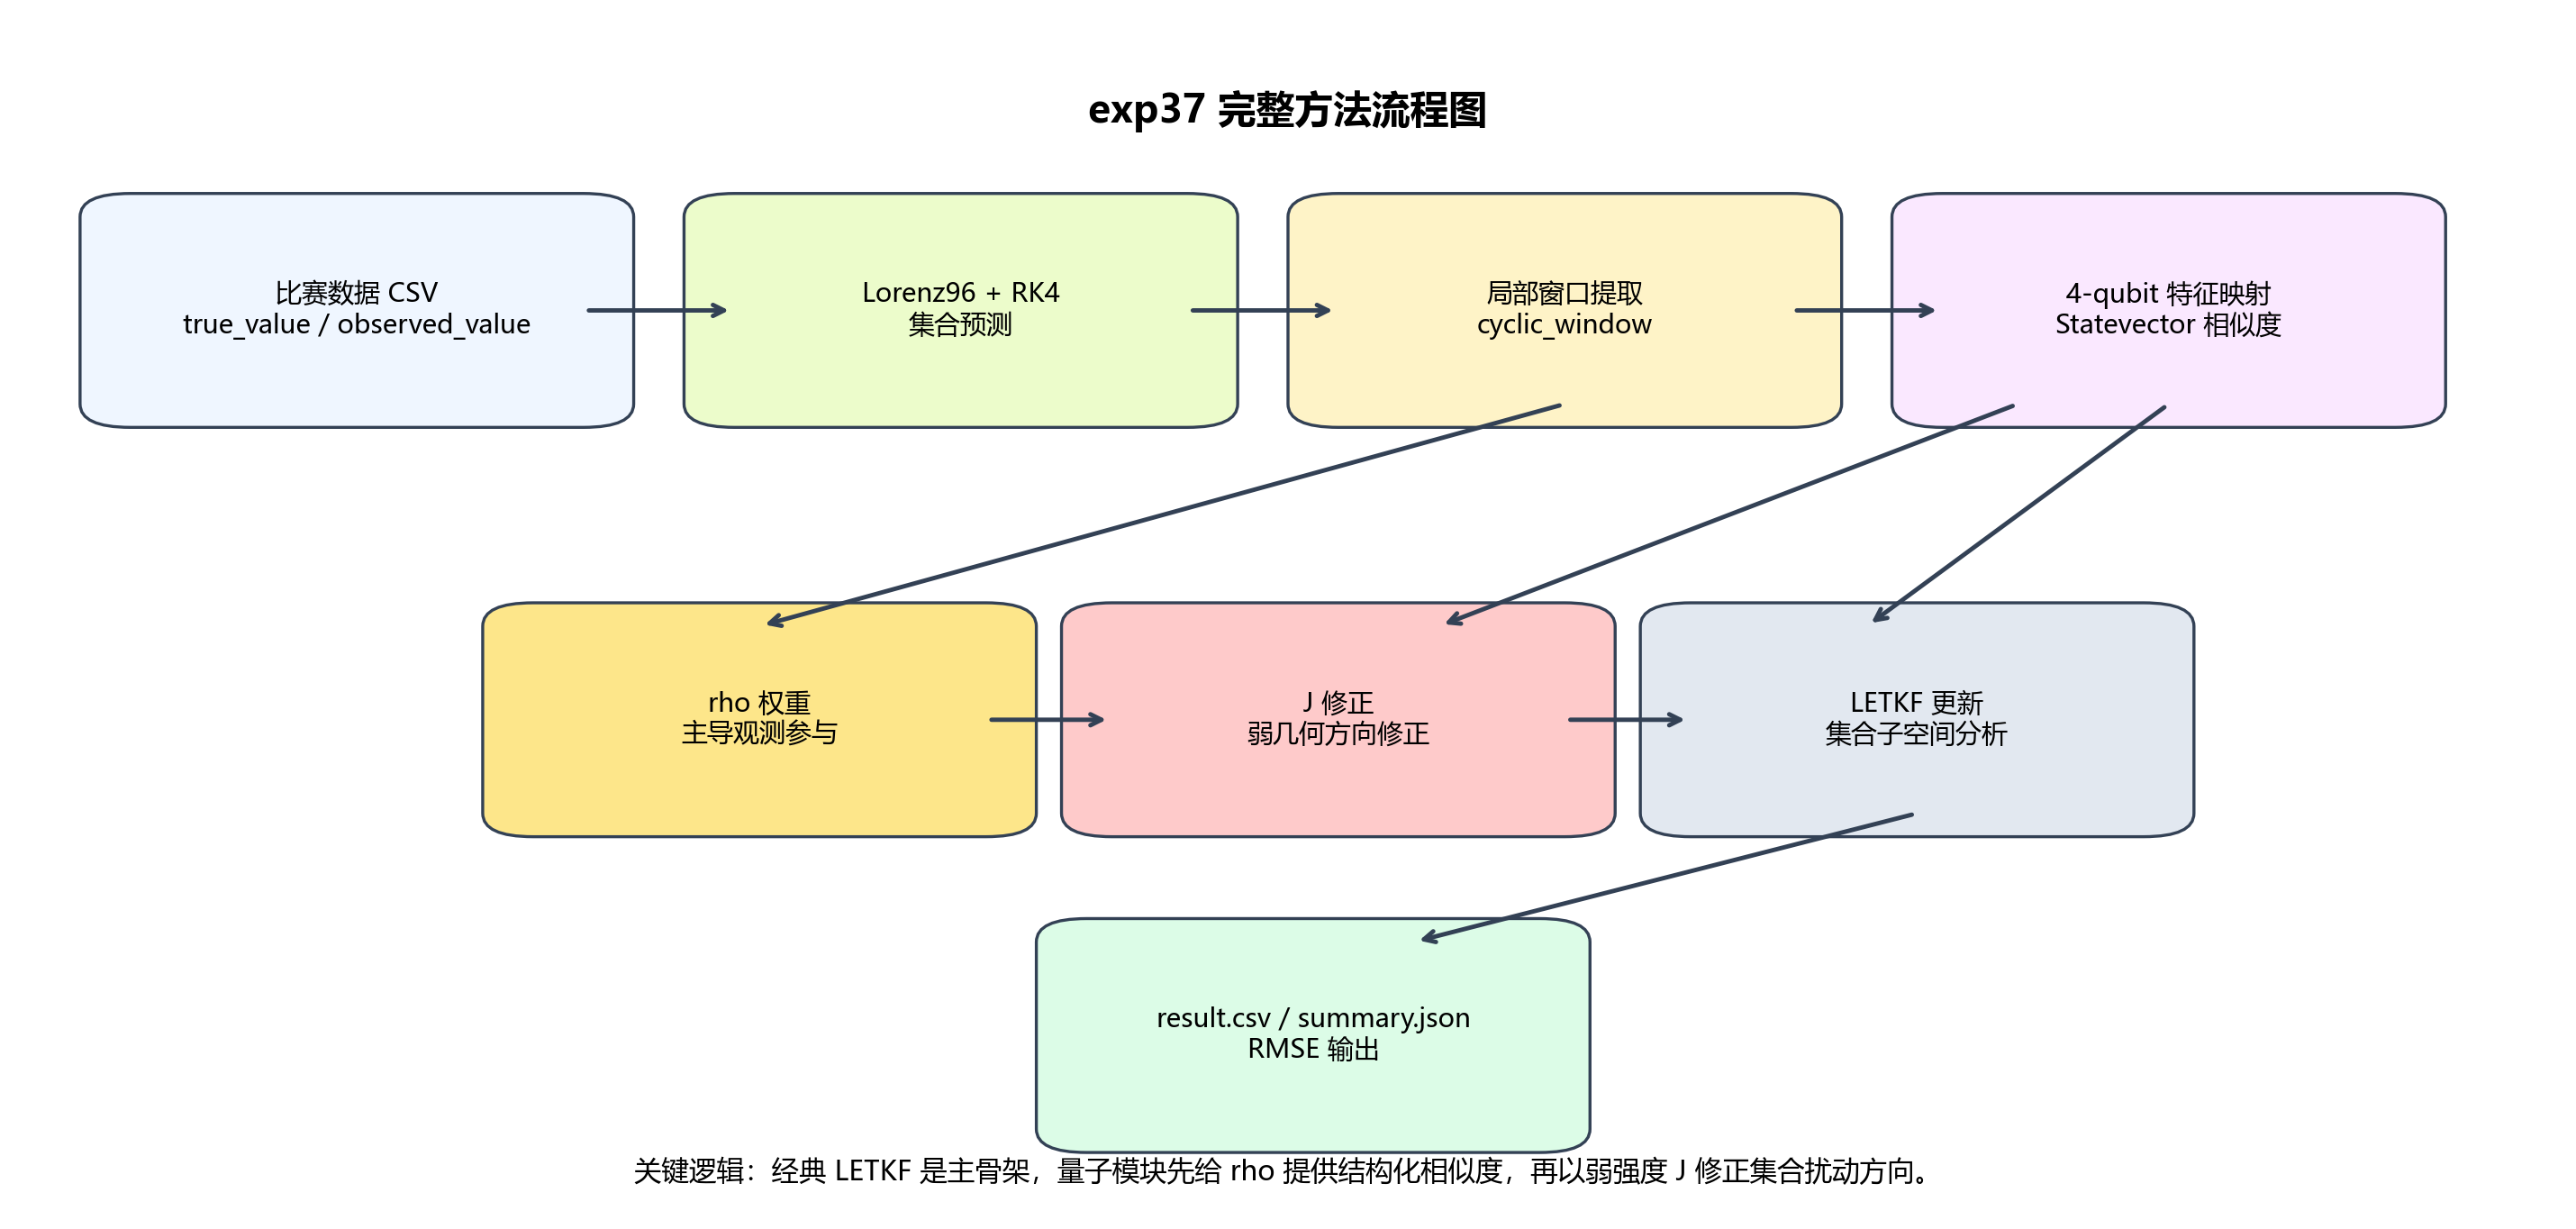
\includegraphics[width=0.9\linewidth]{figures/exp37_method_flowchart.png}
\caption{从输入数据到量子相似度、再到 LETKF 更新的整体流程。}
\label{fig:flow}
\end{figure}

图 \ref{fig:flow} 展示了算法的完整数据流。量子模块只负责构造局地相似度与方向信息，真正的状态更新仍由经典 LETKF 完成，这也是本文保持稳定性的关键。也正因为如此，本文的方法重点不是“让量子模块做更多事情”，而是“让量子模块在最合适的地方介入”。

图 \ref{fig:flow} 还揭示了一个常被忽略的事实：本文算法不是把量子模块附着在流程末端做后处理，而是把它安放在局地权重形成与扰动方向修正之间的关键位置。这个位置选择非常重要。若量子模块放在更外层，它只能扮演参数搜索器；若放在更内层并直接主导分析更新，又容易造成不稳定。将其放在“局地结构判别”这一中间层，既能发挥量子表示能力，又不会破坏经典同化器的主更新机制。

\begin{figure}[htbp]
\centering
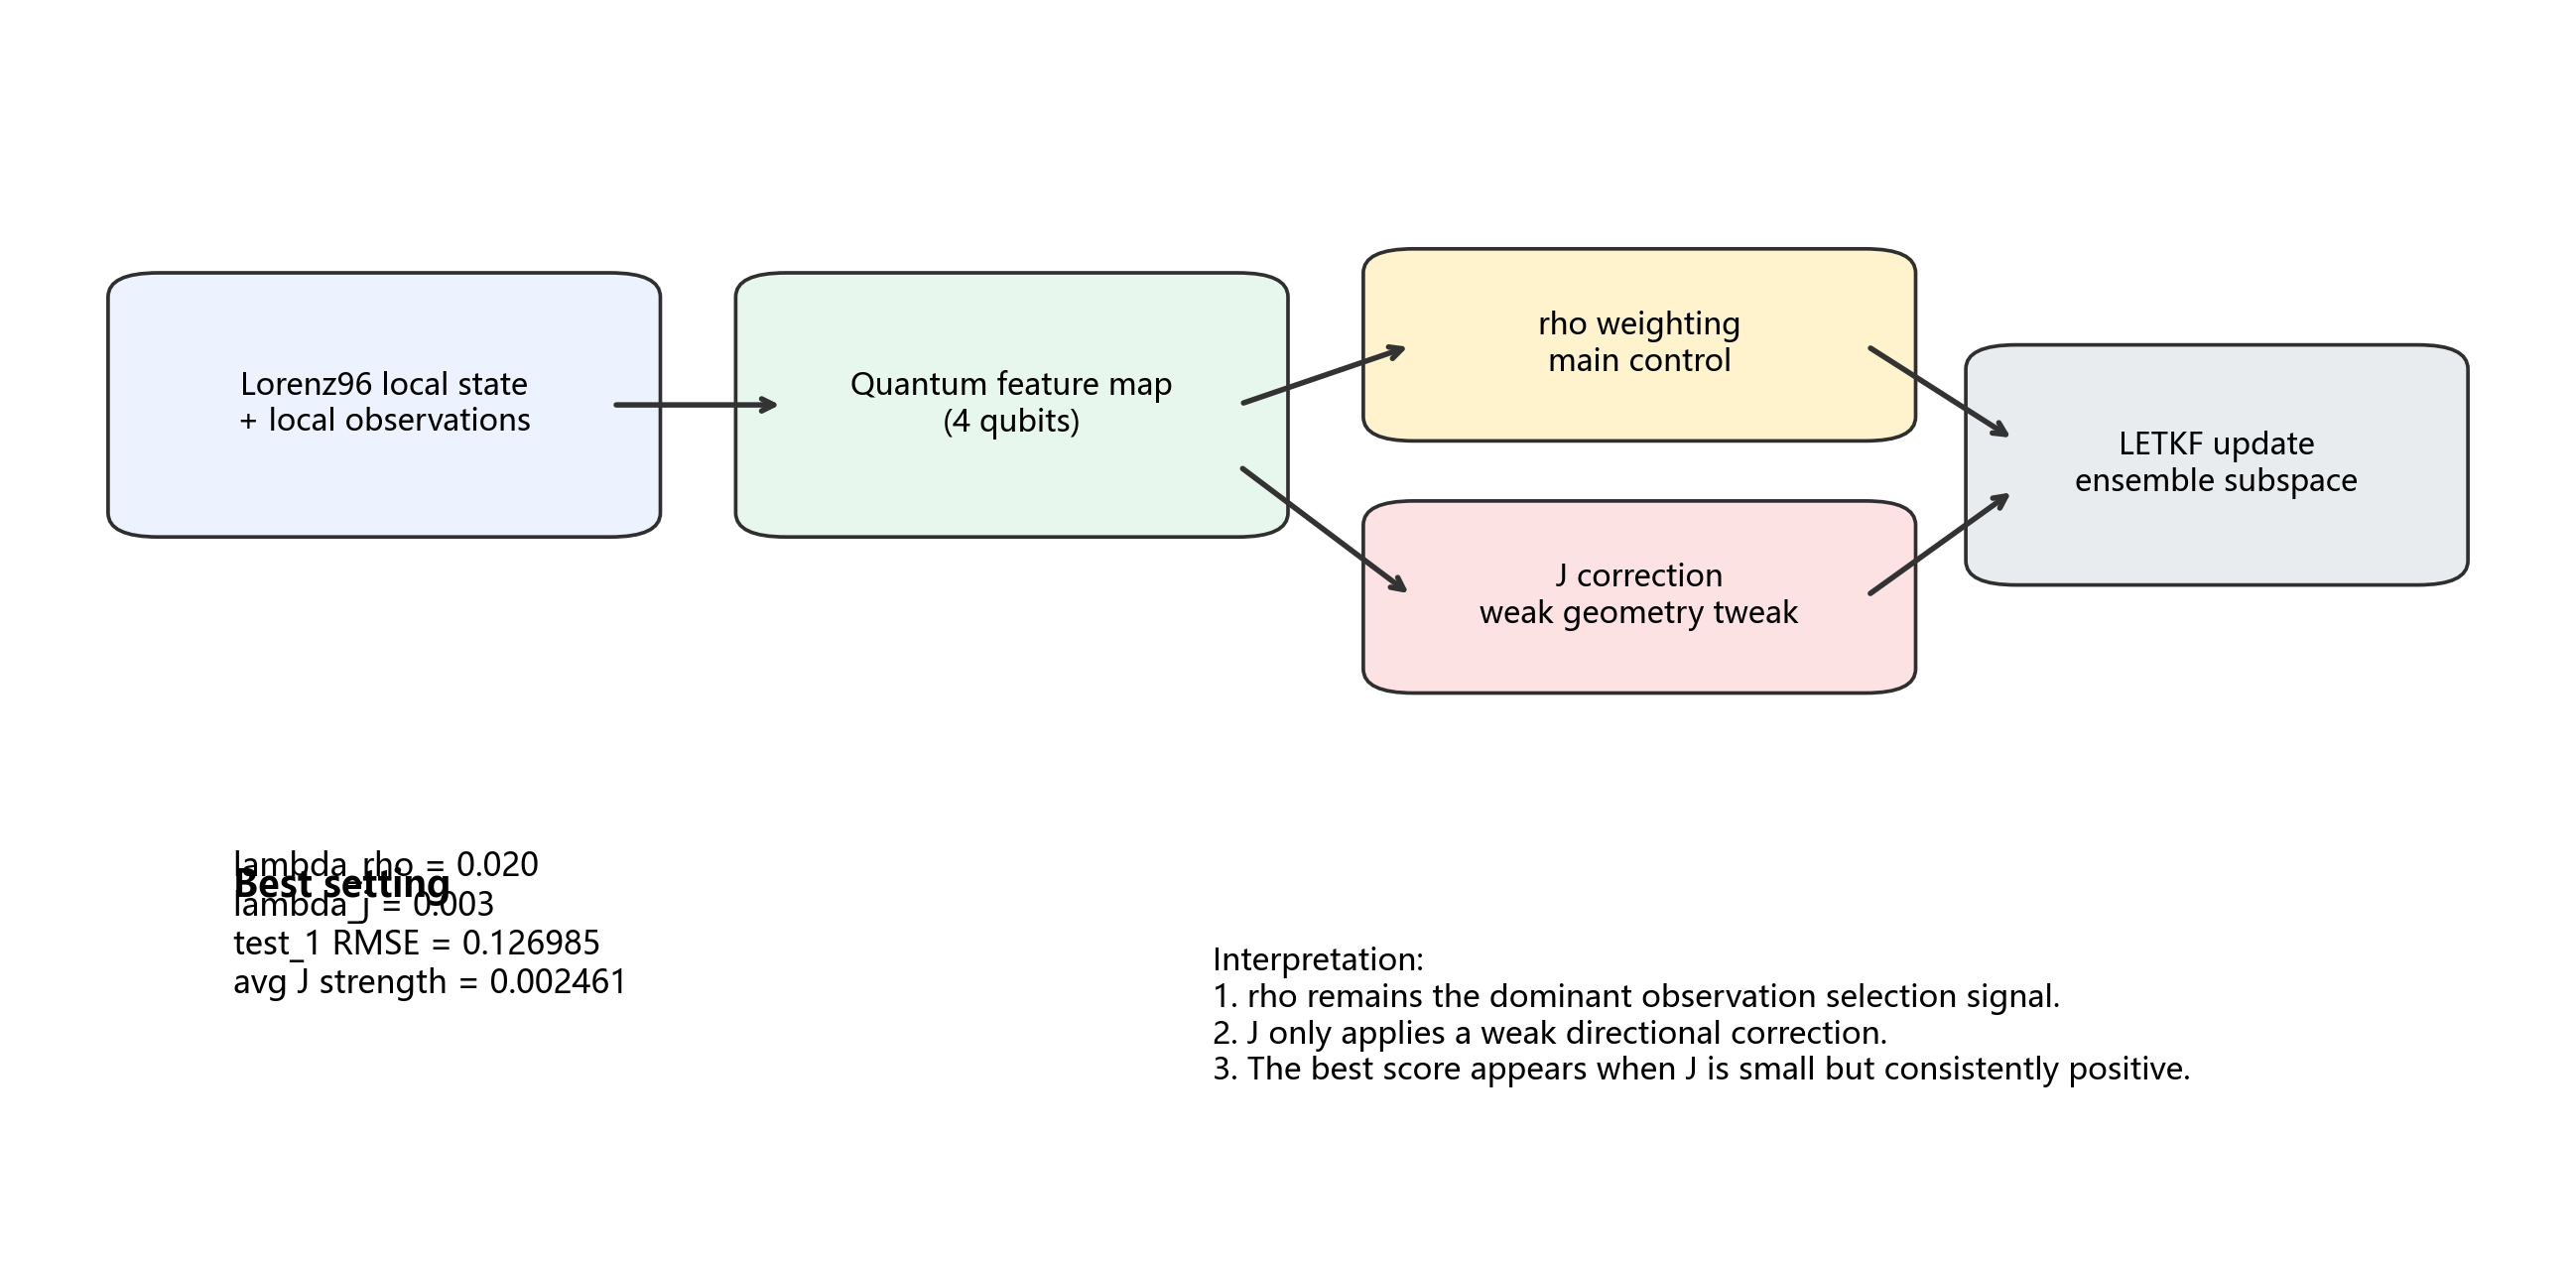
\includegraphics[width=0.92\linewidth]{figures/exp37_method_schematic.png}
\caption{exp37 方法结构示意图，展示 $\rho$ 主导与 $J$ 弱修正的接入关系。}
\label{fig:method}
\end{figure}

图 \ref{fig:method} 比流程图更进一步，它把本文算法最核心的控制思想展示了出来：$\rho$ 融合负责提供主要的局地观测加权，而 $J$ 修正只做小幅方向性调节。也就是说，本文并不是同时把多个量子信号大幅注入更新公式，而是建立了“主调制 + 弱修正”的双层结构。这个结构的优点在于，一旦某个局地窗口上的量子信号不够稳定，损害也会被限制在弱修正层，而不会直接冲击整个分析更新。

为避免口号化叙述，这里把算法中最关键的三个量重新明确写出。第一，局地量子融合权重为
\begin{equation}
w_{ij}=\mathrm{Norm}\!\left(\rho_{ij}\big((1-\lambda_\rho)+\lambda_\rho k_q(i,j)\big)\right),
\end{equation}
其中 $\mathrm{Norm}(\cdot)$ 表示裁剪后再归一化到均值为 $1$ 的操作。第二，局地模式为
\begin{equation}
m_i=\mathrm{NormVec}(Y_i q_i),
\end{equation}
其中 $q_i$ 由量子相似度矩阵得到。第三，$J$ 修正项为
\begin{equation}
J_i=c_i m_i,\qquad c_i=\frac{\langle \tilde{x}_i,m_i\rangle}{\|\tilde{x}_i\|_2+\varepsilon},
\end{equation}
并据此得到修正后的扰动
\begin{equation}
\tilde{x}_i^{(J)}=\tilde{x}_i+\lambda_J J_i.
\end{equation}
当前 exp37 脚本没有额外硬门控条件，等价于使用连续耦合系数 $c_i$ 作为内生强度控制；因此本文报告中的“弱 $J$ 修正”应理解为连续弱修正，而不是阈值门控修正。后续 gated 变体属于扩展实验，不纳入本报告主结果表。

\subsection{算法步骤}
\begin{itemize}
\item 用观测初始化集合，并按 Lorenz96 动力学推进每个集合成员；
\item 对每个状态维度提取局地状态窗口和局地观测窗口；
\item 通过量子特征映射计算状态窗口与各观测窗口之间的量子相似度；
\item 将量子相似度与距离先验进行弱融合，形成局地观测权重；
\item 利用局地量子模式与集合扰动的耦合系数构造连续弱 $J$ 修正；
\item 用修正后的局地权重和扰动信号执行 LETKF 分析更新。
\end{itemize}

上述流程中，最重要的不是单个公式本身，而是“先加权、再弱修正”的顺序。我们先让量子相似度温和调节观测权重，再利用局地模式耦合关系修正集合方向，这样可以避免量子信息一次性过强进入更新公式，引发数值不稳定。

这一顺序实际上对应了本文对量子信号可信度的分层判断。观测权重调制属于相对温和的介入，因为它仍然保留经典距离先验作为底座；而集合方向修正则更敏感，因为它直接影响分析增量的几何方向。因此，本文把方向修正限制为与耦合系数 $c_i$ 和 $\lambda_J$ 成正比的小幅连续修正，而不是直接替换整个更新方向。这种“分层介入、逐步放权”的策略，是本文从前期失败实验中总结出来的重要经验。

\subsection{伪代码}
\noindent\textbf{算法 1：量子弱融合 LETKF}
\begin{quote}
\small\ttfamily
输入：观测序列 $y_{1:T}$，集合规模 $N$，局地半径 $r$，融合系数 $\lambda_\rho,\lambda_J$\\
初始化集合 $E_0$\\
for $t=1$ to $T$ do\\
\quad 用 Lorenz96 推进每个集合成员\\
\quad for 每个状态维度 $i$ do\\
\qquad 提取状态窗口 $s_i$ 与局地观测窗口集合 $\{o_j\}$\\
\qquad 计算量子相似度 $k_q(i,j)$\\
\qquad 计算弱融合权重 $w_{ij}$\\
\qquad 构造局地量子模式 $m_q$\\
\qquad 计算耦合系数 $c_i$，得到 $J_i=c_i m_q$\\
\qquad 构造修正后扰动 $\tilde{x}_i^{(J)}=\tilde{x}_i+\lambda_J J_i$\\
\qquad 用 $w_{ij}$ 和修正后的扰动执行 LETKF 更新\\
\quad end for\\
\quad 输出当前分析场均值\\
end for
\end{quote}

从伪代码可以看出，本文算法并非简单在 LETKF 前后插入一个量子黑箱，而是把量子相似度计算、弱融合权重构造、局地模式提取、$J$ 修正构造和分析更新整合为一条连续的数据流。这样的设计使算法具备两个优点。第一，每一步都可以单独解释和可视化，因此方法不是黑箱。第二，每一步都可以单独消融和替换，因此本文的实验路线天然支持解释性验证和机制分析，而不仅仅是最终指标比较。
